\chapter{Apprendre des demandes de crédit à la consommation} \label{chap1}
\minitoc

\epigraph{Les hommes mentent mais pas les chiffres.}{Kaaris}

Ce chapitre est destiné à poser les bases de l'apprentissage statistique dans le cadre des crédits à la consommation. On introduira dans une première partie la terminologie consacrée du crédit à la consommation avant de s'attarder plus en détails, dans une seconde partie, sur l'état de l'art industriel du \textit{Credit Scoring} à travers une étude bibliographique et la pratique de \gls{cacf}. On clotûrera le chapitre par une troisième partie, la plus traditionnelle pour débuter un manuscrit de thèse, à savoir l'état de l'art académique de l'apprentissage statistique, en nous limitant bien entendu aux cas d'usage spécifiques aux crédits à la consommation mis en exergue dans les deux premières parties de ce chapitre.

\section{Le marché du crédit à la consommation : quels enjeux ?} \label{chap1:sec1}

S'agissant d'une thèse CIFRE, il apparaît comme nécessaire de planter le décor industriel de la problématique. Dans cette première partie, on verra succintement le coeur du métier de \gls{cacf}, les produits que l'entreprise propose et l'environnement dans lequel elle s'insert.

\subsection{Qu'est-ce qu'un crédit à la consommation ?}

La définition légale en a été donnée en~\nameref{chap_intro}. En pratique, on peut distinguer trois produits de crédit à la consommation.


Le premier d'entre eux, le \gls{creditclassique}, est le produit historique. De la même manière qu'un crédit immobilier, le client emprunte une somme fixe qui lui est attribuée au moment du financement et qu'il rembourse selon un échéancier défini à l'avance (taux et nombre de mensualités fixes). D'un point de vue statistique, le traitement est relativement simple : que ce soit à l'octroi, pour déterminer le risque du client, ou au cours de la vie du dossier, pour provisionner les pertes potentielles, tout est connu à l'avance. Il suffit en quelque sorte de vérifier le paiement de la mensualité à la date prévue. Il convient également de préciser que certains crédits classiques sont dits \glspl{creditaffecte}, c'est-à-dire qu'ils financent un bien précis et identifié, de sorte que le prêt transite directement de l'organisme prêteur au vendeur (un concessionnaire par exemple). Par ailleurs, la mise en défaut du crédit entraîne généralement une procédure de recouvrement de la dette qui peut se solder, dans le cas d'un \gls{creditaffecte}, par la récupération du bien par un huissier. Là encore, d'un point de vue statistique, il paraît indispensable de consigner les caractéristiques du bien sous-jacent afin d'intégrer sa valeur résiduelle récupérable en cas de défaut.


Le second produit, développé à partir de 1965 en France et ayant connu une forte croissance depuis~\cite{ducourant2009credit} mais néanmoins bien moins répandu en Europe qu'aux Etats-Unis par exemple~\cite{credit_cards_country}, est le \gls{creditrenouvelable}. Un capital dit accordé ou autorisé est attribué au demandeur qui peut utiliser tout ou partie de ce montant et le rembourse à un taux et par mensualités dépendants tous deux de la proportion du capital consommé. Au fur et à mesure du remboursement du capital emprunté, le capital ``empruntable'', c'est-à-dire la différence entre le capital accordé et le capital emprunté à date, se reconstitue et de nouvelles utilisations sont possibles, toujours dans la limite du capital accordé au départ. D'un point de vue statistique à nouveau, plusieurs problèmes se posent du fait du caractère intrinsèquement aléatoire de l'utilisation ou non de tout ou partie de la ligne de crédit accordée. Plus précisément, ce produit présente un risque important porté par deux facteurs : premièrement, le taux élevé attire des clients risqués, au taux de défaut plus élevé que pour un crédit classique par exemple ; deuxièmement, ces crédits portent un risque dit de hors-bilan très fort, puisqu'à tout moment, l'ensemble des crédits accordés mais non utilisés et donc non comptabilisés ``au bilan'', c'est-à-dire comme une dette du client envers l'établissement bancaire, peuvent être utilisés et faire défaut. La mauvaise quantification de ce risque est à présent reconnu comme un important catalyseur de la récente crise financière \cite{karim2013off}.


Enfin, la \gls{location} a récemment connu un essor important~\cite{peden_2018}. D'abord concentrée sur le secteur automobile, elle se développe actuellement pour les produits électroniques (smartphones notamment) et même plus récemment pour des produits plus insolites comme les matelas~\cite{dicharry_2017}. Comme le \gls{creditaffecte}, il est important de prendre en compte les données du bien loué afin d'évaluer le risque que porte ce produit, la difficulté supplémentaire reposant sur l'éventualité de l'exercice de l'hypothétique option d'achat.

De cette partie, deux considérations statistiques doivent retenir notre attention : d'abord, ces différents produits nécessitent des traitements différents dans la mesure où leur risque est intrinsèquement différent ; ensuite, les données disponibles pour chacun de ces produits diffèrent : par exemple, les données du produit financé ne sont disponibles que pour les \glspl{creditaffecte} et les \glspl{location}. Cette dernière notion de ``blocs'' de variables est au coeur du chapitre~\ref{chap6}.

%\subsection{Quels sont les acteurs de ce marché ?}
%Au même titre que la partie précédente, cette partie ne se veut pas une analyse du marché du crédit à la consommation mais 

\subsection{Crédit Agricole Consumer Finance}

\gls{cacf} opère dans de nombreux pays. En France, c'est principalement à travers la marque Sofinco que sont commercialisés les crédits à la consommation pour lesquels il existe une relation directe entre \gls{cacf} et le client (dite B2C), par exemple lorsqu'un demandeur se rend directement sur le site internet \href{https://www.sofinco.fr}{sofinco.fr}.

Par ailleurs, de nombreux crédits à la consommation sont distribués à travers un réseau de partenaires, qui jouent le rôle d'intermédiaires (on parle alors de B2B) : concessionnaires automobile, distributeurs d'électroménager, etc.

Enfin, \gls{cacf} faisant partie du groupe Crédit Agricole, de nombreuses agences bancaires distribuent des crédits à la consommation à leur clientèle bancarisé, par l'intermédiaire des gestionnaires de compte.

Là encore, on constate que les spécificités des canaux de distribution des crédits impactent grandement la collecte des données et leur traitement statistique. En effet, les informations collectées sur le client, le produit et éventuellement l'apporteur d'affaires sont différentes selon le canal.

Dans la partie suivante, la méthodologie présentée est spécifique à \gls{cacf} ; il pourra néanmoins être admis que, dans les grandes lignes, cette méthodologie est similaire à la concurrence d'une part, et à la pratique d'autres pays (européens du moins) puisque la législation sur la protection et le traitement des données est sensiblement similaire (du fait de l'entrée en vigueur récente de la GDPR) et le fait que les établissements bancaires possèdent généralement des filiales dans plusieurs pays d'Europe et y font appliquer la même méthodologie.

% disclaimer
%Par ailleurs, les données réelles utilisées pour illustrer les méthodologies statistiques présentées dans ce manuscrit sont la propriété de \gls{cacf}.

\section{Le \textit{Credit Scoring} : état de l'art de la pratique industrielle} \label{chap1:sec2}

Cette partie vise à présenter la pratique actuelle en matière de \textit{Credit Scoring} et pose un certain nombre de questions statistiques dont certaines ont été traitées dans cette thèse, d'autres trouvent des réponses (parfois partielles) dans la littérature et dont certaines références sont données à titre informatif mais ne sont pas développées dans ce manuscrit ; enfin, certaines questions ne trouvent \textit{a priori} pas de réponse immédiate dans la littérature et sont autant de matière à de futurs travaux dans le domaine !

\subsection{Collecte des données}

La partie précédente a mis en exergue la pluralité des sources de données. La figure~\ref{fig:souscription} présente par exemple le formulaire de souscription en vigueur pour un crédit automobile auprès de Sofinco \textit{via} son site web. Dans cet exemple, des données socio-démographiques et du véhicule à financer sont demandées. Pour un client, elles sont notées $\glssymbol{bx} = (\glssymbol{x}_j)_1^d$ dans la suite. Ces informations sont de nature continue, c'est-à-dire $\glssymbol{x}_j \in \glssymbol{R}$, ou catégorielle, c'est-à-dire que l'on se donne, à titre d'exemple, un encodage ``Métier = technicien'' $\rightarrow \glssymbol{x}_j = 1$, ``Métier = ouvrier'' $\rightarrow \glssymbol{x}_j = 2$, \dots de telle sorte que l'on considère que $\glssymbol{x}_j \in \glssymbol{N}_{o_j}$, où $o_j$ représente le nombre de modalités de $x_j$ et sans notion d'ordre. Cela permettra d'alléger les notations en lieu et place de noter le support de chaque variable catégorielle différemment.

\begin{figure}
\centering 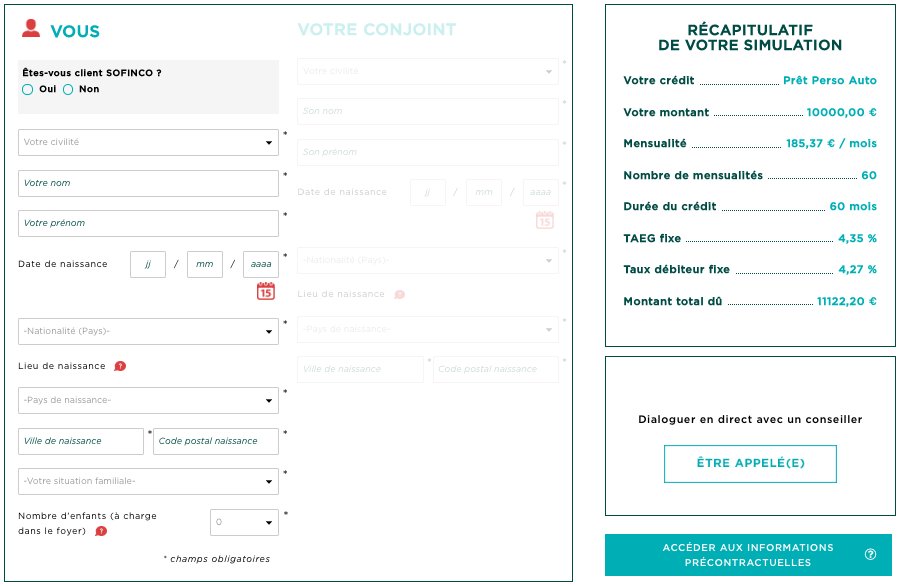
\includegraphics[width=15cm]{figures/chapitre1/souscription.png}
\caption{\label{fig:souscription} Formulaire de souscription d'un crédit automobile Sofinco.}
\end{figure}

On considère que ces caractéristiques sont une réalisation du vecteur aléatoire de design $\glssymbol{bX} = (\glssymbol{Xj})_1^d \in \mathcal{X}$ sur un espace probabilisé $(\Omega,\mathcal{A},\mathbb{P})$, que l'on observe sur l'ensemble des $n$ demandeurs de crédit à la consommation pour former, dans la littérature consacrée au \textit{machine learning}, la matrice de design $\glssymbol{bbx} = (\glssymbol{xij})_{1 \leq i \leq n, 1 \leq j \leq d}$. En accord avec ce qui précède, on se limite au cas $\mathcal{X} \subseteq\glssymbol{R}^d$.

A ce stade, deux remarques importantes doivent être faites : d'abord, la partie précédente a montré qu'en fonction du produit demandé et du canal de la demande, une partie de ces caractéristiques peuvent être absentes. Par ailleurs, ces informations étant, à ce stade, déclaratives (des contrôles supplémentaires peuvent avoir lieu en fonction du montant demandé par exemple), elles sont associées à un degré de certitude variable, la tentation étant grande, afin de s'assurer de l'attribution du crédit, de déformer la réalité de ses charges, ses revenus, etc. En synthèse, le tableau~\ref{tab:design} présente un exemple simplifié de matrice de design en \textit{Credit Scoring}. En pratique un tel tableau structuré est directement mis à disposition des statisticiens de \gls{cacf} à travers le logiciel de traitement statistique SAS.

%\begin{table}
%\centering
%\begin{scriptsize}
%\begin{tabular}{p{1.4cm}|p{1.7cm}|p{1cm}|p{0.8cm}|p{1.4cm}|p{0.9cm}}
%Travail & Logement & Durée d'emploi & Enfants & Statut familial & Salaire \\
%\hline
%Ouvrier qualifié & Propriétaire & 20 & 3 & Veuf & 30 000  \\
%Technicien & En location & Manquant & 1 & Concubinage & \textcolor{orange}{1700}  \\
%Technicien spécialisé & Accédant & 5 & 0 & Divorcé & \textcolor{red}{4000}  \\
%Cadre & Par l'employeur & 8 & 2 & Célibataire & \textcolor{orange}{2700}  \\
%Employé & En location & 12 & 2 & Marié & \textcolor{red}{1400}  \\
%Ouvrier & Par la famille & 2 & 0 & Célibataire & \textcolor{green}{1200}  \\
%\end{tabular}
%\end{scriptsize}
%\caption{\label{tab:design} Exemple simplifié de caractéristiques de demandeurs de crédit : présence de valeurs manquantes, extrêmes, et d'un degré d'erreur de mesure différent (\textcolor{green}{faible erreur de mesure}, \textcolor{orange}{erreur de mesure moyenne}, \textcolor{red}{forte erreur de mesure} : déformation de la vérité par le client).}
%\end{table}

\begin{table}
\centering
%\begin{scriptsize}
%\begin{tabular}{p{1.4cm}|p{1.7cm}|p{1cm}|p{0.8cm}|p{1.4cm}|p{0.9cm}}
\begin{tabular}{l|l|l|l|l|l}
Travail & Logement & Durée d'emploi & Enfants & Statut familial & Salaire \\
\hline
Ouvrier qualifié & Propriétaire & 20 & 3 & Veuf & 30 000  \\
Technicien & En location & Manquant & 1 & Concubinage & {1700}  \\
Technicien spécialisé & Accédant & 5 & 0 & Divorcé & {4000}  \\
Cadre & Par l'employeur & 8 & 2 & Célibataire & {2700}  \\
Employé & En location & 12 & 2 & Marié & {1400}  \\
Ouvrier & Par la famille & 2 & 0 & Célibataire & {1200}  \\
\end{tabular}
%\end{scriptsize}
\caption{\label{tab:design} Exemple simplifié de caractéristiques de demandeurs de crédit : présence de valeurs manquantes ou extrêmes.}
\end{table}

\subsection{Préparation des données et segmentation}

Le tableau~\ref{tab:design} fait apparaître deux problèmes bien connus en statistique : la gestion des observations manquantes et celle des valeurs extrêmes (\textit{outliers}).

% et l'erreur de mesure, relative à la mauvaise déclaration des demandeurs. Ce dernier problème ne sera pas traité ici.

Concernant les observations manquantes, deux stratégies différentes peuvent être employées. \gls{cacf} réalise une ``segmentation'' de sa clientèle, de sorte que, à titre d'exemple, plusieurs modèles statistiques spécialisés à un sous-ensemble de la population totale peuvent être employés, chacun d'eux bénéficiant alors de données complètes. On pourra par exemple se limiter aux demandeurs de crédit automobile afin d'exploiter les données du véhicule à financer, qui sont alors toutes renseignées. Le processus de choix des ``segments'', \textit{i.e.}\ la partition des lignes de $\glssymbol{bbx}$ sur lesquels développer des modèles séparés, est basé soit sur l'histoire de l'entreprise (par exemple, un modèle spécifique aux crédits automobiles a pu être développé au début de la commercialisation de ce produit), soit sur des heuristiques très simples. On détaillera ce problème en chapitre~\ref{chap6}.

L'autre pré-traitement répandu dans le milieu du \textit{Credit Scoring} pour faire face aux données manquantes et aux valeurs extrêmes est la discrétisation (pour les variables continues uniquement). Cela consiste à transformer une variable continue dont certaines observations sont manquantes en une variable catégorielle dont chaque modalité correspond à un intervalle de la variable continue d'origine et / ou au fait que l'observation d'origine était manquante. Un exemple de discrétisation de la variable ``Âge du client'' est visible en figure~\ref{tab:disc_ex} ; ainsi, le fait que l'observation soit manquante est considérée comme une information à part entière et les valeurs extrêmes sont regroupées dans le dernier intervalle. Les mécanismes de données manquantes seront discutés en chapitre~\ref{chap2}. Le processus de discrétisation est discuté en détail au chapitre~\ref{chap4}.

\begin{table}
\centering
%\begin{scriptsize}
%\begin{tabular}{p{1.4cm}|p{1.4cm}|p{1.4cm}|p{1.4cm}|p{1.4cm}|p{1.4cm}|p{1.4cm}}
\begin{tabular}{l|l|l|l|l|l|l}
Âge du client & 18 & Manquant & 47 & 25 & 35 & 61 \\
\hline
Âge discrétisé & 18-30 \& Manquant & 18-30 \& Manquant & 45-$\infty$ & 18-30 & 30-45 & 45-$\infty$ \\
\end{tabular}
%\end{scriptsize}
\caption{\label{tab:disc_ex} Exemple de variable continue discrétisée.}
\end{table}

\`A présent, on dispose de données rendues complètes sur l'ensemble des demandeurs de crédit et l'on souhaite prédire le niveau de risque présenté par un nouveau demandeur. Il convient donc dans un premier temps de quantifier le risque de chaque échantillon de la matrice de design $\glssymbol{bbx}$.

\subsection{Critère à modéliser} \label{subsec:critere}

L'institut financier emprunte de l'argent sur les marchés à un taux relativement faible et le redistribue aux demandeurs de crédit qu'il juge profitables, c'est-à-dire susceptible de rembourser cette dette. Il y a donc un système d'acceptation, reposant sur un ensemble de règles automatiques et potentiellement une étude humaine. On considère que le mécanisme qui conduit au financement \textit{in fine} de la demande de crédit est aléatoire, noté $Z$ et prenant les valeurs f (pour les clients dont la demande est financée) et nf (pour les non-financés).

Il convient de noter ici que les différents processus qui conduisent à un non financement du dossier sont très nombreux : interruption / rétractation du demandeur, refus automatique (endettement, \gls{score} existant, \dots) ou refus d'un conseiller clientèle. On y reviendra très brièvement au chapitre~\ref{chap2}.

En essence, il est souhaitable de mesurer la profitabilité de chaque crédit, par exemple en actualisant les remboursements et les pertes générés par chaque client à la date de déblocage des fonds, et en déduisant l'ensemble des coûts (financement, traitement, recouvrement, \dots). En pratique, peu d'institutions procèdent ainsi malgré quelques travaux récents~\cite{finlay2010credit}.

En conséquence, on sélectionne généralement 12 mois de dossiers de demandes de crédit pour s'affranchir de phénomènes de saisonnalité et on observe le mois suivant la date de financement de chaque dossier si la mensualité a été remboursée. On répète le processus jusqu'à un horizon de 12 à 24 mois selon la disponibilité des données. On dispose alors pour chaque client d'une série temporelle qui indique si le remboursement mensuel a été effectué ou non. On cherche ensuite à se ramener à une seule variable aléatoire cible $\glssymbol{Y} \in \{0,1\}$ qualifiant un client ``bon'' par $Y=1$ ou ``mauvais'' par $Y=0$. L'heuristique actuellement utilisée est la suivante :
\begin{itemize}
\item Pour un horizon $T=\{6,12,18,24\}$ mois et $I = \{0,\dots,6\}$ impayés consécutifs,
\begin{itemize}
\item Construire le tableau des \textit{Roll Rates}, dont un exemple est donné en tableau~\ref{tab:impayes}.

On cherche le nombre d'impayés consécutifs $I$ au-delà duquel la proportion de dossiers se dégradant (et donc fortement susceptibles de générer des pertes) est ``importante'', généralement au-delà de 50 \%. 
\item Tracer le graphique d'``horizon du risque'', dont un exemple est donné en figure~\ref{fig:courbe_horizon}.

On cherche un point d'inflexion sur cette courbe, qui traduirait le fait qu'au-delà d'un certain horizon $T$, la proportion de dossiers ``mauvais'' n'évolue plus et l'on considère que tous les ``mauvais'' clients sont déjà identifiés.
\end{itemize}
\item Choisir le couple $(T,I)$ qui répond au mieux aux critères ci-dessus et permet d'avoir un nombre significatif de dossiers ``mauvais''. Il faut garder à l'esprit que plus l'on choisit un horizon $T$ faible et / ou un nombre élevé d'impayés consécutifs $I$, plus la proportion $\hat{\pi}_0$ (l'estimateur de la moyenne pour $\pi_i = p(Y=i)$) de dossiers ``mauvais'' par rapport aux dossiers ``bons'' devient faible. On note dans la suite, de manière classique, $\pi_i = p(Y=i)$. Or, on veut éviter au maximum les nombreux problèmes que génèrent des classes déséquilibrées en classification supervisée~\cite{sun2009classification}.
\end{itemize}

\begin{figure}
\centering
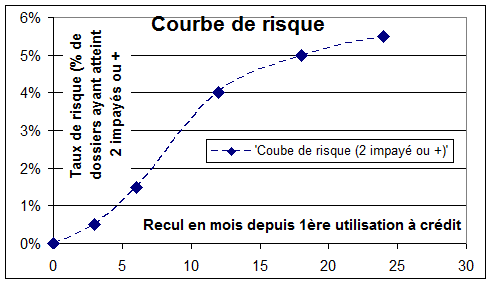
\includegraphics[width=10cm]{figures/chapitre1/courbe_risque.png}
\caption{\label{fig:courbe_horizon} Exemple de courbe d'horizon risque : proportion de ``mauvais'' clients (2 impayés consécutifs) en fonction du nombre de mensualités observées.}
\end{figure}

\begin{table}
\centering
%\fbox{%
%\begin{scriptsize}
%\begin{tabular}{p{1.4cm}|p{1.7cm}|p{1.7cm}|p{1.7cm}}
\begin{tabular}{l|l|l|l}
Impayés consécutifs & Amélioration & Stabilité & Dégradation \\
\hline
0 & 0 \% & 95 \% & 5 \%  \\
1 & 60 \% & 10 \% & 30 \%  \\
2 & 10\% & 30 \% & \textcolor{red}{60 \%} \\
3 & 5\% & 25 \% & {70 \%} \\
4 & 5\% & 15 \% & {80 \%} \\
5 & 5\% & 5 \% & {90 \%} \\
\end{tabular}
%\end{scriptsize}
\caption{\label{tab:impayes} Exemple d'évolution de dossiers à différents niveaux d'impayés.} 
\end{table}

%% schéma temporel

% listing ?

% figure horizon risque exemple

Pour des raisons pratiques et historiques, on choisit généralement $T=12$ mois et $I = 2$ impayés consécutifs. On considère donc comme ``mauvais'' ($Y=0$) les dossiers financés ayant eu plus de 2 mensualités impayées consécutives dans les 12 mois qui ont suivi leur financement, comme ``bons'' ($Y=1$) les dossiers n'ayant pas eu d'impayés, comme ``indéterminés'' les dossiers ayant eu 1 impayé, et on exclut tous les dossiers non financés ($Z=\nf$). On a alors le vecteur de réponse $\glssymbol{bby}$ dont un exemple est donné en tableau~\ref{tab:rep_ex}.

\begin{table}
\centering
%\begin{scriptsize}
%\begin{tabular}{p{1.4cm}|p{1.4cm}|p{1.4cm}|p{1.4cm}|p{1.4cm}|p{1.4cm}|p{1.4cm}}
\begin{tabular}{|c|c|c|c|c|c|c|}
\hline
$y$ & 1 & Manquant - Non-financé& 0 & Manquant - Indéterminé & 0 & 1 \\
\hline
\end{tabular}
%\end{scriptsize}
\caption{\label{tab:rep_ex} Exemple de vecteur $\glssymbol{bby}$ de qualification du risque des clients.}
\end{table}

On en conclut que la performance de remboursement n'est observable que pour les clients financés non indéterminés, que l'on va assimiler dans la suite à ceux pour lesquels $Z=\f$, problème qui fait l'objet du chapitre~\ref{chap2}. Toujours-est-il qu'à présent, on dispose de données $(\glssymbol{bbx},\glssymbol{bby})$ complètes grâce auxquelles on souhaite apprendre une règle de décision, appelée \gls{score} et discernant, parmi les futurs demandeurs de crédit, les ``bons'' des ``mauvais'' clients.

\subsection{L'apprentissage d'une règle de décision}

Malgré l'existence de nombreux modèles statistiques permettant de prédire $\glssymbol{Y}$ connaissant les caractéristiques $\glssymbol{bX}$ d'un client et que nous discuterons en partie~\ref{chap1:sec3}, la régression logistique est très largement utilisée en \textit{Credit Scoring}~\cite{thomas2000survey}. Plusieurs travaux empiriques ont suggéré que du fait de la nature des données ``classiques'' en \textit{Credit Scoring}, \textit{i.e.}\ faible nombre de covariables et classes très mélangées (en particulier, absence de frontière de séparation linéaire entre ``bons'' et ``mauvais'' clients), aucun autre modèle de classification supervisée ne produit de résultats significativement supérieurs à la régression logistique sur les données à disposition de leurs auteurs respectifs (se référer par exemple à~\cite{hand1997statistical,baesens2003benchmarking,brown2012experimental}).

Le modèle de régression logistique, contrairement à ce que son nom suggère, est un modèle de classification qui impose une structure particulière de loi de probabilité d'une variable aléatoire cible binaire $\glssymbol{Y}$ conditionnellement à des covariables explicatives $\glssymbol{bX} \in \mathcal{X}=\glssymbol{R}^d$ donnée par :
\begin{equation} \label{eq:logit}
\text{logit}[p(Y=1 | \glssymbol{bX}=\glssymbol{bx}, \glssymbol{bth})] = \ln \frac{p(Y=1 | \glssymbol{bX}=\glssymbol{bx}, \glssymbol{bth})}{1-p(Y=1 | \glssymbol{bX}=\glssymbol{bx}, \glssymbol{bth})} = \glssymbol{bth}' \times (1,\glssymbol{bx})
\end{equation}
Le vecteur $\glssymbol{bth} = (\theta_0,\dots,\theta_d) \in \Theta = \glssymbol{R}^{d+1}$ est appelé paramètre. Le coefficient $\theta_0$ définit le biais, c'est-à-dire $\text{logit}[p(Y=1 | \glssymbol{bX}=\bm{0}, \glssymbol{bth})]$. Cette relation est ensuite inversée afin d'obtenir la probabilité d'être ``bon'' sachant les caractéristiques d'un client et le paramètre $\glssymbol{bth}$ : $$p(Y=1 | \glssymbol{bX}=\glssymbol{bx}, \glssymbol{bth}) = \frac{1}{1+\exp({-\glssymbol{bth}' \times (1,\glssymbol{bx}))}},$$ et dont des exemples de courbe sont donnés en figure~\ref{fig:logit}.

\begin{figure}
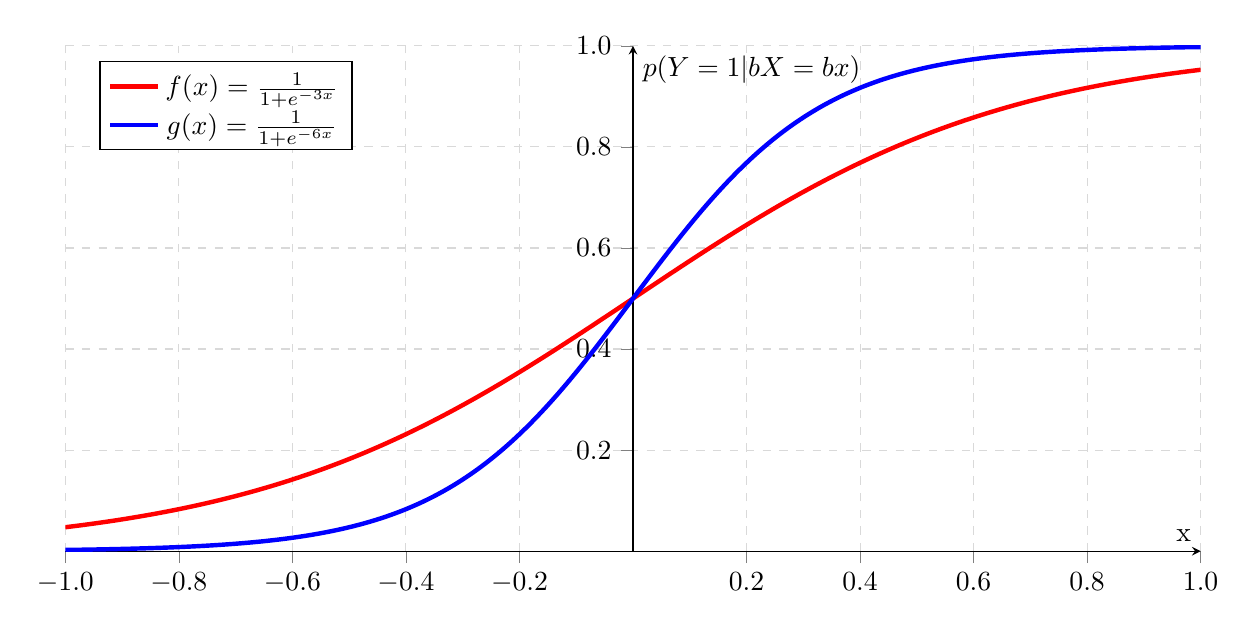
\begin{tikzpicture}
    \begin{axis}[
    	legend pos=north west,
        axis x line=middle,
        axis y line=middle,
        x tick label style={/pgf/number format/fixed,
                            /pgf/number format/fixed zerofill,
                            /pgf/number format/precision=1},
        y tick label style={/pgf/number format/fixed,
                            /pgf/number format/fixed zerofill,
                            /pgf/number format/precision=1},
        grid = major,
        width=16cm,
        height=8cm,
        grid style={dashed, gray!30},
        xmin=-1,     % start the diagram at this x-coordinate
        xmax= 1,    % end   the diagram at this x-coordinate
        ymin= 0,     % start the diagram at this y-coordinate
        ymax= 1,   % end   the diagram at this y-coordinate
        %axis background/.style={fill=white},
        xlabel=x,
        ylabel={$p(\glssymbol{Y}=1 | \glssymbol{bX} = \glssymbol{bx})$},
        tick align=outside,
        enlargelimits=false]
      % plot the stirling-formulae
      \addplot[domain=-1:1, red, ultra thick,samples=500] {1/(1+exp(-3*x))};
      \addplot[domain=-1:1, blue, ultra thick,samples=500] {1/(1+exp(-6*x))};
      \addlegendentry{$f(x)=\frac{1}{1+e^{-3x}}$}
      \addlegendentry{$g(x)=\frac{1}{1+e^{-6x}}$}
    \end{axis}
\end{tikzpicture}
\caption{\label{fig:logit} Deux exemples de courbes logistiques à une variable explicative sans paramètre de biais.}
\end{figure}

% Discuter variables catégorielles
On peut facilement étendre ce modèle aux variables catégorielles $X_j \in \glssymbol{NO}$ en procédant à un encodage \textit{one-hot}, c'est-à-dire en créant une matrice à $o_j$ colonnes dont l'entrée $(i,k)$ vaut 1 si $x_{i,j} = k$, $1 \leq i \leq n$ et $1 \leq k \leq o_j$, 0 sinon. Par exemple pour $o_j=3$, un encodage possible est :
$$ \left( \begin{array}{c} 1 \\ 2 \\ 3 \end{array} \right) \to \left( \begin{array}{ccc} 1 & 0 & 0 \\ 0 & 1 & 0 \\ 0 & 0 & 1 \end{array} \right).$$
Cette pratique conduit cependant à une sur-paramétrisation : la somme des colonnes vaut 1 et la matrice n'est donc pas de plein-rang, ce qui pose un problème pour l'estimation de $\glssymbol{bth}$ comme nous le verrons en partie~\ref{chap1:sec3} ; il faut donc ``supprimer'' une colonne en considérant une modalité dite de référence (\textit{i.e.}\ pour laquelle le coefficient est nul). Cet encodage est implicite dans de nombreux logiciels statistiques, si bien que l'on notera les coefficients de régression logistique associés à chaque valeur d'une variable catégorielle $X_j$ en exposant : $\theta_j^{1},\dots,\theta_j^{o_j}$. On considérera la dernière modalité comme référence, d'où $\theta_j^{o_j} = 0$.

En fonction du risque que l'institut financier est prêt à prendre, on décide d'un \gls{cut}, c'est-à-dire d'une probabilité de défaut au-delà de laquelle on refuse la demande de crédit. On désigne traditionnellement par \gls{score} la fonction $S(\cdot,\glssymbol{bth}): \glssymbol{bx} \mapsto \glssymbol{bth}' \times (1,\glssymbol{bx})$.

La question du support  de $\glssymbol{bth}$, \textit{i.e.}\ de ses valeurs non nulles, est un problème plus connu sous le nom de ``sélection de variables'' en statistiques comme en \textit{machine learning}. Un coefficient nul témoigne du fait que la variable associée $X_j$, conditionnellement aux autres variables que l'on notera $X_{\{-j\}}$ dans la suite, ne permet pas d'expliquer $Y$. En industrie, il est courant de commencer par sélectionner les variables dont la corrélation avec la variable cible est jugée suffisante. Cette technique univariée ne permet pas de rendre compte de phénomènes multivariées comme la redondance d'information entre covariables ou, à l'inverse, la qualité prédictive d'une variable dont la corrélation avec la cible peut être faible mais qui apporterait une information conditionnellement aux autres variables explicatives. La communauté statistique a donc développé des outils spécifiques à cette question que l'on développera, avec les fondements théoriques des modèles paramétriques comme la régression logistique, en partie~\ref{chap1:sec3}.

\subsection{La métrique de performance}

La métrique utilisée pour comparer la qualité de \glspl{score} (le score ancien et un nouveau score proposé par exemple) est traditionnellement l'indice de Gini, qui est en fait directement lié à l'aire sous la courbe (AUC) ROC. Cette courbe représente la sensibilité d'un classificateur binaire (\textit{i.e.}\ la proportion de ``bons'' clients classés comme ``bons'') en fonction de son antispécificité ($1-$ la spécificité, \textit{i.e.}\ la proportion de ``mauvais'' clients classés comme ``bons''). L'AUC s'interprète de plusieurs manières, dont par exemple la probabilité qu'un ``bon'' (tiré aléatoirement parmi les ``bons'') ait un score plus élevé qu'un ``mauvais'' (tiré aléatoirement parmi les ``mauvais''). Un exemple de courbe ROC est donné en figure~\ref{fig:ROC}.

\begin{figure}
\centering \scalebox{.8}{% Created by tikzDevice version 0.10.1 on 2018-08-02 16:56:45
% !TEX encoding = UTF-8 Unicode
\begin{tikzpicture}[x=1pt,y=1pt]
\definecolor{fillColor}{RGB}{255,255,255}
\path[use as bounding box,fill=fillColor,fill opacity=0.00] (0,0) rectangle (289.08,289.08);
\begin{scope}
\path[clip] (  0.00,  0.00) rectangle (289.08,289.08);
\definecolor{drawColor}{RGB}{0,0,0}

\node[text=drawColor,anchor=base,inner sep=0pt, outer sep=0pt, scale=  1.00] at (156.54,  9.60) {Specificity};

\node[text=drawColor,rotate= 90.00,anchor=base,inner sep=0pt, outer sep=0pt, scale=  1.00] at ( 16.80,156.54) {Sensitivity};
\end{scope}
\begin{scope}
\path[clip] (  0.00,  0.00) rectangle (289.08,289.08);
\definecolor{drawColor}{RGB}{0,0,0}

\path[draw=drawColor,line width= 0.4pt,line join=round,line cap=round] ( 49.20, 49.20) --
	(263.88, 49.20) --
	(263.88,263.88) --
	( 49.20,263.88) --
	( 49.20, 49.20);

\path[draw=drawColor,line width= 0.4pt,line join=round,line cap=round] (255.93, 49.20) -- ( 57.15, 49.20);

\path[draw=drawColor,line width= 0.4pt,line join=round,line cap=round] (255.93, 49.20) -- (255.93, 43.20);

\path[draw=drawColor,line width= 0.4pt,line join=round,line cap=round] (216.17, 49.20) -- (216.17, 43.20);

\path[draw=drawColor,line width= 0.4pt,line join=round,line cap=round] (176.42, 49.20) -- (176.42, 43.20);

\path[draw=drawColor,line width= 0.4pt,line join=round,line cap=round] (136.66, 49.20) -- (136.66, 43.20);

\path[draw=drawColor,line width= 0.4pt,line join=round,line cap=round] ( 96.91, 49.20) -- ( 96.91, 43.20);

\path[draw=drawColor,line width= 0.4pt,line join=round,line cap=round] ( 57.15, 49.20) -- ( 57.15, 43.20);

\node[text=drawColor,anchor=base,inner sep=0pt, outer sep=0pt, scale=  1.00] at ( 57.15, 27.60) {1.0};

\node[text=drawColor,anchor=base,inner sep=0pt, outer sep=0pt, scale=  1.00] at ( 96.91, 27.60) {0.8};

\node[text=drawColor,anchor=base,inner sep=0pt, outer sep=0pt, scale=  1.00] at (136.66, 27.60) {0.6};

\node[text=drawColor,anchor=base,inner sep=0pt, outer sep=0pt, scale=  1.00] at (176.42, 27.60) {0.4};

\node[text=drawColor,anchor=base,inner sep=0pt, outer sep=0pt, scale=  1.00] at (216.17, 27.60) {0.2};

\node[text=drawColor,anchor=base,inner sep=0pt, outer sep=0pt, scale=  1.00] at (255.93, 27.60) {0.0};

\path[draw=drawColor,line width= 0.4pt,line join=round,line cap=round] ( 49.20, 57.15) -- ( 49.20,255.93);

\path[draw=drawColor,line width= 0.4pt,line join=round,line cap=round] ( 49.20, 57.15) -- ( 43.20, 57.15);

\path[draw=drawColor,line width= 0.4pt,line join=round,line cap=round] ( 49.20, 96.91) -- ( 43.20, 96.91);

\path[draw=drawColor,line width= 0.4pt,line join=round,line cap=round] ( 49.20,136.66) -- ( 43.20,136.66);

\path[draw=drawColor,line width= 0.4pt,line join=round,line cap=round] ( 49.20,176.42) -- ( 43.20,176.42);

\path[draw=drawColor,line width= 0.4pt,line join=round,line cap=round] ( 49.20,216.17) -- ( 43.20,216.17);

\path[draw=drawColor,line width= 0.4pt,line join=round,line cap=round] ( 49.20,255.93) -- ( 43.20,255.93);

\node[text=drawColor,rotate= 90.00,anchor=base,inner sep=0pt, outer sep=0pt, scale=  1.00] at ( 34.80, 57.15) {0.0};

\node[text=drawColor,rotate= 90.00,anchor=base,inner sep=0pt, outer sep=0pt, scale=  1.00] at ( 34.80, 96.91) {0.2};

\node[text=drawColor,rotate= 90.00,anchor=base,inner sep=0pt, outer sep=0pt, scale=  1.00] at ( 34.80,136.66) {0.4};

\node[text=drawColor,rotate= 90.00,anchor=base,inner sep=0pt, outer sep=0pt, scale=  1.00] at ( 34.80,176.42) {0.6};

\node[text=drawColor,rotate= 90.00,anchor=base,inner sep=0pt, outer sep=0pt, scale=  1.00] at ( 34.80,216.17) {0.8};

\node[text=drawColor,rotate= 90.00,anchor=base,inner sep=0pt, outer sep=0pt, scale=  1.00] at ( 34.80,255.93) {1.0};
\end{scope}
\begin{scope}
\path[clip] ( 49.20, 49.20) rectangle (263.88,263.88);
\definecolor{drawColor}{RGB}{169,169,169}

\path[draw=drawColor,line width= 0.4pt,line join=round,line cap=round] ( 49.20, 49.20) -- (263.88,263.88);
\definecolor{drawColor}{RGB}{0,0,0}

\path[draw=drawColor,line width= 0.8pt,line join=round,line cap=round] (255.93,255.93) --
	(252.11,255.93) --
	(248.28,255.93) --
	(244.46,255.93) --
	(240.64,255.93) --
	(236.82,255.93) --
	(232.99,255.93) --
	(229.17,255.93) --
	(225.35,255.93) --
	(221.53,255.93) --
	(217.70,255.93) --
	(213.88,255.93) --
	(210.06,255.93) --
	(206.23,255.93) --
	(202.41,255.93) --
	(198.59,255.93) --
	(194.77,255.93) --
	(190.94,255.93) --
	(187.12,255.93) --
	(183.30,255.93) --
	(183.30,251.79) --
	(179.48,251.79) --
	(175.65,251.79) --
	(175.65,247.65) --
	(171.83,247.65) --
	(171.83,243.51) --
	(168.01,243.51) --
	(168.01,239.36) --
	(164.19,239.36) --
	(160.36,239.36) --
	(160.36,235.22) --
	(160.36,231.08) --
	(156.54,231.08) --
	(152.72,231.08) --
	(148.89,231.08) --
	(145.07,231.08) --
	(141.25,231.08) --
	(137.43,231.08) --
	(137.43,226.94) --
	(133.60,226.94) --
	(129.78,226.94) --
	(125.96,226.94) --
	(125.96,222.80) --
	(122.14,222.80) --
	(118.31,222.80) --
	(114.49,222.80) --
	(114.49,218.66) --
	(114.49,214.52) --
	(110.67,214.52) --
	(106.85,214.52) --
	(103.02,214.52) --
	( 99.20,214.52) --
	( 99.20,210.38) --
	( 99.20,206.23) --
	( 99.20,202.09) --
	( 99.20,197.95) --
	( 99.20,193.81) --
	( 99.20,189.67) --
	( 99.20,185.53) --
	( 99.20,181.39) --
	( 95.38,181.39) --
	( 91.55,181.39) --
	( 91.55,177.25) --
	( 91.55,173.10) --
	( 91.55,168.96) --
	( 91.55,164.82) --
	( 87.73,164.82) --
	( 83.91,164.82) --
	( 83.91,160.68) --
	( 83.91,156.54) --
	( 83.91,152.40) --
	( 80.09,152.40) --
	( 80.09,148.26) --
	( 76.26,148.26) --
	( 76.26,144.12) --
	( 76.26,139.98) --
	( 76.26,135.83) --
	( 72.44,135.83) --
	( 72.44,131.69) --
	( 72.44,127.55) --
	( 72.44,123.41) --
	( 72.44,119.27) --
	( 72.44,115.13) --
	( 68.62,115.13) --
	( 68.62,110.99) --
	( 68.62,106.85) --
	( 68.62,102.70) --
	( 68.62, 98.56) --
	( 68.62, 94.42) --
	( 68.62, 90.28) --
	( 68.62, 86.14) --
	( 68.62, 82.00) --
	( 68.62, 77.86) --
	( 68.62, 73.72) --
	( 68.62, 69.57) --
	( 64.80, 69.57) --
	( 64.80, 65.43) --
	( 64.80, 61.29) --
	( 60.97, 61.29) --
	( 60.97, 57.15) --
	( 57.15, 57.15);

\node[text=drawColor,anchor=base west,inner sep=0pt, outer sep=0pt, scale=  1.00] at (156.54,149.65) {AUC: 0.812};
\end{scope}
\end{tikzpicture}
}
\caption{\label{fig:ROC} Exemple de courbe ROC sur un petit jeu de données simulées et valeur de l'AUC correspondante.}
\end{figure}

Il faut remarquer à ce stade que ce critère est à la fois différent de celui optimisé par la régression logistique, que nous verrons en détails dans la partie suivante, et de l'objectif industriel de maximiser le profit, soit directement par l'usage de variables de nature financière~\cite{finlay2010credit}, soit indirectement par le choix d'un \gls{cut} approprié. Néanmoins, une étude empirique~\cite{finlay2009we} montre que la maximisation de ces différents objectifs est \textit{a priori} relativement équivalent, la qualité prédictive de différents modèles maximisant chacun de ces objectifs étant similaires sur le jeu de données considéré par l'auteur. On suppose cette équivalence dans la suite et sauf indication contraire, les résultats sur données réelles sont donnés en Gini, dont on essaiera de donner un intervalle de confiance selon la méthode développée dans~\cite{cortes2005confidence}.



\subsection{Suivi temporel de la performance du \gls{score}}

Les changements de contexte économique, agissant à la fois sur les variables explicatives $\glssymbol{bX}$ (l'inflation ou le passage à l'euro impacte l'échelle des salaires par exemple) et la variable cible (la récession entraîne l'augmentation des impayés), la performance du \gls{score}, selon la métrique précédemment décrite, évolue au cours du temps. Naturellement, cette évolution est la plupart du temps à la baisse puisque la fonction de \gls{score} apprise s'éloigne de la vérité. Par ailleurs, comme vu en partie~\ref{subsec:critere}, l'apprentissage du \gls{score} nécessite environ 30 mois de recul, auxquels peuvent s'ajouter un délai de mise en production. Dès lors, le statisticien voit émerger deux questions : premièrement, quels sont les ``signes'' indiquant qu'une refonte, c'est-à-dire la mise en place d'un nouveau modèle prédictif, est nécessaire ? Deuxièmement, est-il possible de construire un modèle prédictif ``robuste'' à ce problème, communément désigné par \textit{population drift} dans la littérature~\cite{hand1997statistical} ?

En pratique, seuls la baisse de performance d'un \gls{score} et / ou son ancienneté importante (5 à 10 ans) conduisent à sa refonte et l'aspect temporel n'est pas pris en compte dans la construction ou l'utilisation des \glspl{score}.

\medskip

En conclusion, le \textit{Credit Scoring} repose sur des bases statistiques qui soulèvent de nombreuses questions, dont certaines trouvent dans le milieu industriel une réponse \textit{ad hoc}, très empirique, qu'il convient de formaliser. La partie suivante plonge l'apprentissage du \gls{score} dans le contexte de l'apprentissage statistique.

\section{Apprentissage statistique : fondements théoriques du \textit{Credit Scoring}} \label{chap1:sec3}

Après cette mise en situation industrielle qui aura mis en avant les approximations statistiques et autres heuristiques actuellement utilisées dans le milieu, il convient de formaliser les concepts introduits en partie~\ref{chap1:sec2}. Cette partie s'inspire librement d'introductions de plusieurs ouvrages, dont le bien connu~\citetitle*{friedman2001elements}~\cite{friedman2001elements}.

\subsection{Mécanisme de génération des données}

On note $p$ la \gls{pdf} de $(\glssymbol{bX},Y)$ et $\pd(\cdot | \glssymbol{bx})$ la loi de probabilité de $Y$ sachant $\glssymbol{bx}$, qui s'obtient à partir de $p$ et de la relation de Bayes: $$\pd(\cdot | \glssymbol{bx}) = \frac{p(\glssymbol{bx},y)}{p(\glssymbol{bx})},$$ que l'on désignera par ``oracle'' dans la suite. On aimerait ``retrouver'' cette loi par calcul, or elle est inconnue (si elle était connue, le problème serait résolu !), et on a uniquement accès à un $n$-échantillon $\mathcal{T}_n = (\glssymbol{bbx},\glssymbol{bby})$ dont on note la loi de probabilité (uniforme) $\ps$.

Imaginons un instant que $\pd(\cdot | \glssymbol{bx})$ soit connu. Une première approche consiste en quelque sorte à exprimer notre connaissance de cette loi en la forçant à appartenir à un modèle (ou à une famille de modèles). Autrement dit, on suppose que $\pd(\cdot | \glssymbol{bx})$ appartient à un ensemble (très) restreint des lois possibles. Si l'on note $\mathcal{B}(\mathcal{X} \times \mathcal{Y})$ la tribu borélienne sur $\mathcal{X} \times \mathcal{Y}$, alors $p$, dont $\pd$ est un sous-produit, est l'une des nombreuses mesures de probabilités possibles sur l'espace mesurable $(\mathcal{X} \times \mathcal{Y},\mathcal{B}(\mathcal{X} \times \mathcal{Y}))$. Comme énoncé plus haut, dans le cadre du \textit{Credit Scoring}, on s'intéresse au modèle de \gls{lr}~\eqref{eq:logit} noté $p_{\glssymbol{bth}}(\cdot | \glssymbol{bx})$ dans la suite. Dès lors, une formulation simple du problème consiste à se donner une notion de distance entre $p_{\text{data}}(\cdot | \glssymbol{bx})$ et $p_{\glssymbol{bth}}(\cdot | \glssymbol{bx})$ afin d'estimer le ``meilleur'' paramètre $\glssymbol{bth}^\star$ au sens de cette ``distance''. Un bon candidat est la divergence de Kullback-Leibler~\cite{kullback1951information} :
\begin{equation} \label{eq:KL}
\glssymbol{KL}(p_{\text{data}}(\cdot | \glssymbol{bx})||p_{\glssymbol{bth}}(\cdot | \glssymbol{bx})) = \sum_{y \in \{0,1\}} p_{\text{data}}(y | \glssymbol{bx}) \ln \left( \frac{p_{\text{data}}(y | \glssymbol{bx})}{p_{\glssymbol{bth}}(y | \glssymbol{bx})} \right)
\end{equation}
Cette divergence est donnée pour une valeur particulière $\glssymbol{bx}$ de $\glssymbol{bX}$. Or, l'institut financier voudrait que le modèle $p_{\glssymbol{bth}}(\cdot | \glssymbol{bx})$ soit similaire à $\pd(\cdot | \glssymbol{bx})$ en moyenne pour tous ses clients, soit $${\glssymbol{bth}}^\star = \argmin_{\glssymbol{bth}} \mathbb{E}_{\glssymbol{bX}} [\glssymbol{KL}(p_{\text{data}}(\cdot | \glssymbol{bx})||p_{\glssymbol{bth}}(\cdot | \glssymbol{bx}))].$$ Comme $\glssymbol{KL}(\pd(\cdot | \glssymbol{bx})||p_{\glssymbol{bth}}(\cdot | \glssymbol{bx})) \geq 0$, on peut voir cette opération comme une projection de la loi $\pd(\cdot | \glssymbol{bx})$ dans l'espace du modèle (ou de la famille de modèles) comme sur la figure~\ref{fig:projection}. Cette interprétation géométrique permet d'affirmer que si $\min_{\glssymbol{bth}} \mathbb{E}_{\glssymbol{bX}} [\glssymbol{KL}(p_{\text{data}}(\cdot | \glssymbol{bx})||p_{\glssymbol{bth}}(\cdot | \glssymbol{bx}))] = 0$, alors on a $p_{\text{data}}(\cdot | \glssymbol{bx}) = p_{\glssymbol{bth}^\star}(\cdot | \glssymbol{bx}) \; \forall \: \glssymbol{bx}$. Dans ce cas, on parlera dans la suite de ``vrai modèle'' ; dans le cas contraire, de ``modèle mal spécifié'' (anglicisme de \textit{misspecified model}).

\begin{figure}
\begin{center}
\resizebox{0.8\textwidth}{4.7cm}{
\begin{tikzpicture}[scale=1.1,every node/.style={minimum size=1cm},on grid]

	% Real level
	\begin{scope}[
		yshift=-120,
		every node/.append style={yslant=\yslant,xslant=\xslant},
		yslant=\yslant,xslant=\xslant
	] 
		% The frame:
		\draw[black, dashed, thin] (0,0) rectangle (7,7); 
		% Agents:
		\draw[fill=red]  
			%(5,2) circle (.1) % Firms
			(2,2) circle (.1); % Households
		% Flows:
		%\draw[-latex,thin, blue] 
			%(2,2.2) to (2,4); % Labour Powers
		%\draw[-latex,thin, blue]
			%(4.85,1.85) to (4,1); % Wages
		 % Labels:
		\fill[black]
			(0.5,6.5) node[right, scale=2.5] {Espace $\Theta$}	
			(2.1,1.9) node[below,scale=2]{$\glssymbol{bth}^\star$};

	\end{scope}
	
	% 2 vertical lines for linking agents on the 2 levels
	%\draw[thin, dashed, red](.8,1.75) to (3.8,-0.32);
	\draw[thin, dashed, red](.8,1.75) to (.8,-1.8);
	
    % Draw right angle scheme
    \draw(.8,-1.6) to (1,-1.6);
    \draw(1,-1.6) to (1,-1.8);


	% Monetary level
	\begin{scope}[
		yshift=-20,
		every node/.append style={yslant=0,xslant=0},
		yslant=\yslant,xslant=\xslant
	]
		 % Agents:
		\draw [fill=olive]
			(2,2) circle (.1); % Households
		 % Labels:
		\fill[black]
			(2.2,2.4) node[right,scale=2]{\textcolor{olive}{$\pd(y|x)$}};
        \fill[red]
			(0.85,0.35) node [right, scale=1.5] {Biais de modèle};	

	\end{scope} 
\end{tikzpicture}
}
\end{center}
\caption{\label{fig:projection} Vision géométrique du biais de modèle.}
\end{figure}

N'ayant accès à $\pd(\cdot | \glssymbol{bx})$ qu'à travers un échantillon, il nous faut développer un critère empirique à partir du critère théorique (on parle aussi de critère asymptotique) donné ici.

\subsection{Minimisation du risque empirique et maximum de vraisemblance}

On peut réécrire $\glssymbol{KL}(p_{\text{data}}(\cdot|\glssymbol{bx})||p_{\glssymbol{bth}}(\cdot|\glssymbol{bx}))$ pour faire apparaître un terme indépendant de $p_{\glssymbol{bth}}$ :
\[ \glssymbol{KL}(p_{\text{data}}(\cdot|\glssymbol{bx})||p_{\glssymbol{bth}}(\cdot|\glssymbol{bx})) = \underbrace{\sum_{y \in \{0,1\}} p_{\text{data}}(y|\glssymbol{bx}) \ln [p_{\text{data}}(y|\glssymbol{bx})]}_{\perp p_{\glssymbol{bth}}} - \underbrace{\sum_{y \in \{0,1\}} p_{\text{data}}(y|\glssymbol{bx}) \ln [p_{\glssymbol{bth}}(y|\glssymbol{bx})]}_{\mathbb{E}_{\glssymbol{Y}} [\ln[p_{\glssymbol{bth}}(\cdot|\glssymbol{bx})]]}  \]
On va donc naturellement se concentrer sur la maximisation du second terme pour l'ensemble des clients en moyenne, c'est-à-dire $\glssymbol{bth}^\star = \argmax_{\glssymbol{bth}} \mathbb{E}_{\glssymbol{bX}}  [\mathbb{E}_{\glssymbol{Y}} [\ln[p_{\glssymbol{bth}}(\cdot|\glssymbol{bx})]]] = \argmax_{\glssymbol{bth}} \mathbb{E}_{(\glssymbol{bX},\glssymbol{Y}) \sim p} [\ln[p_{\glssymbol{bth}}]]$.

En substituant $p$ pour ${p_{\text{sample}}}$, on approxime l'espérance sur $\mathcal{X} \times \mathcal{Y}$ par l'espérance sur l'échantillon et on obtient le critère $\ell(\theta;\glssymbol{bbx},\glssymbol{bby})$ :
\begin{equation} \label{eq:vraisemblance}
\ell(\glssymbol{bth};\glssymbol{bbx},\glssymbol{bby}) = \sum_{i=1}^n \ln[p_{\glssymbol{bth}}(y_i | \glssymbol{bx}_i) ]
\end{equation}
Ce critère correspond en fait au maximum de vraisemblance : la probabilité d'observer les données $(\glssymbol{bbx},\glssymbol{bby})$ sachant le paramètre $\glssymbol{bth}$. On se place dans le cadre d'un $n$-échantillon i.i.d.\ ce qui est toujours le cas en \textit{Credit Scoring} sous réserve que les crédits observés soient issus de clients différents (ce que l'on supposera dans la suite). L'hypothèse d'indépendance nous permet d'écrire la vraisemblance sous la forme d'un produit : $$\mathcal{L}(\glssymbol{bth};\glssymbol{bbx},\glssymbol{bby}) = p_{\glssymbol{bth}}(y_1,\dots,y_n | \glssymbol{bx}_1,\dots \glssymbol{bx}_n) = \prod_{i=1}^n p_{\glssymbol{bth}}(y_i | \glssymbol{bx}_i).$$ En passant cette expression au logarithme, fonction strictement croissante, on retrouve bien la formulation de $\ell(\glssymbol{bth};\glssymbol{bbx},\glssymbol{bby})$.

Dans la littérature \textit{machine learning}, où l'on minimise plutôt un risque empirique, sous-entendu de ``mauvais classement'' au sens d'une fonction de coût à définir, le maximum de vraisemblance est équivalent au minimum de la ``log loss''. Dans la suite, on préférera la notion de vraisemblance.

Dans le cas de la \gls{lr}~\eqref{eq:logit}, la log-vraisemblance prend la forme suivante :
\[ \ell(\glssymbol{bth};\glssymbol{bbx},\glssymbol{bby}) = \underbrace{\sum_{i=1}^n y_i (\glssymbol{bth}' \times (1,\glssymbol{bx}))}_{\text{fonction affine de } \glssymbol{bth}} - \underbrace{\ln(1 + \exp(\glssymbol{bth}' \times (1,\glssymbol{bx}))}_{\text{log-sum-exp d'une fonction affine de } \glssymbol{bth}} \qedhere \]
Cette fonction est concave et tout maximum local est donc global. 
\begin{proof}
On suppose que $\hat{\glssymbol{bth}}$ est un maximum local ; il y a un voisinage $\mathcal{V}$ de $\hat{\glssymbol{bth}}$ sur lequel $\ell(\hat{\glssymbol{bth}};\glssymbol{bbx},\glssymbol{bby}) \geq \ell(\glssymbol{bth};\glssymbol{bbx},\glssymbol{bby})$ pour tout $\glssymbol{bth} \in \mathcal{V}$. Soit $\tilde{\glssymbol{bth}} \in \bm{\Theta}$ et $0 \leq t \leq 1$. Pour $t$ suffisamment petit, $(1-t)\hat{\glssymbol{bth}} + t \tilde{\glssymbol{bth}}$ est dans $\mathcal{V}$ et la concavité de $\ell$ donne :
\begin{align*}
\ell(\hat{\glssymbol{bth}};\glssymbol{bbx},\glssymbol{bby}) & \geq \ell(t \tilde{\glssymbol{bth}} + (1-t)\hat{\glssymbol{bth}};\glssymbol{bbx},\glssymbol{bby}) \\
& \geq t \ell(\tilde{\glssymbol{bth}};\glssymbol{bbx},\glssymbol{bby}) + (1-t) \ell(\hat{\glssymbol{bth}};\glssymbol{bbx},\glssymbol{bby}) \\
& \geq \ell(\tilde{\glssymbol{bth}};\glssymbol{bbx},\glssymbol{bby})
\end{align*}
\end{proof}

Le ``réflexe'' pour obtenir un maximum local conduit à dériver la fonction de vraisemblance et trouver $\hat{\glssymbol{bth}}$ pour lequel cette dérivé est nulle :
\[ \dfrac{\delta \ell}{\delta \theta_j} (\hat{\glssymbol{bth}};\glssymbol{bbx},\glssymbol{bby})= \sum_{i=1}^n (y_i - p_{\hat{\glssymbol{bth}}}(1|\glssymbol{bx}_i)) x_{i,j} = 0\]

Cependant, contrairement à la régression linéaire où l'on dispose d'une formule close pour l'estimateur du maximum de vraisemblance $\hat{\glssymbol{bth}}$, il n'existe rien de tel pour la \gls{lr} puisque cette équation n'est pas linéaire en $\glssymbol{bth}$ et l'on doit recourir à des algorithmes itératifs, dont le plus connu est la descente de gradient et ses nombreux dérivés.

On désigne le gradient de la log-vraisemblance par rapport à $\glssymbol{bth}$ par $\nabla_{\glssymbol{bth}} \ell = \left( \dfrac{\delta \ell}{\delta \theta_j} \right)_0^d$. L'algorithme de descente de gradient consiste à mettre à jour à l'étape $(s)$ le paramètre $\glssymbol{bth}^{(s)}$ dans la direction qui améliore le critère $\ell(\glssymbol{bth};\glssymbol{bbx},\glssymbol{bby})$ : $$\glssymbol{bth}^{(s+1)} = \glssymbol{bth}^{(s)} + \epsilon \nabla_{\glssymbol{bth}} \ell(\glssymbol{bth}^{(s)};\glssymbol{bbx},\glssymbol{bby}).$$ Une immense littérature est dédiée au choix d'$\epsilon$, appelé \textit{learning rate} en \textit{machine learning} et à d'autres astuces destinées à accélérer la convergence éventuelle vers $\hat{\glssymbol{bth}}$. Cette littérature s'est particulièrement développée dans le cadre des réseaux de neurones, pour lesquels la méthode de Newton, bien adaptée à la \gls{lr} et que l'on développera ci-après, n'est pas tractable.

On note la matrice hessienne de $\ell$ en $\glssymbol{bth}$ par $\mathbf{H}_{\glssymbol{bth}} = \left( \dfrac{\delta \ell}{\delta \theta_j \delta \theta_k} \right)_{1 \leq j,k \leq d}$. Le développement de Taylor, qui revient à considérer que la log-vraisemblance est localement quadratique, donne à l'étape $(s)$ :
\[ \ell(\glssymbol{bth}^{(s+1)};\glssymbol{bbx},\glssymbol{bby}) = \ell({\glssymbol{bth}}^{(s)};\glssymbol{bbx},\glssymbol{bby}) + \nabla_{\glssymbol{bth}} \ell(\glssymbol{bth}^{(s)};\glssymbol{bbx},\glssymbol{bby})' (\glssymbol{bth}^{(s+1)} - {\glssymbol{bth}}^{(s)}) + \dfrac{1}{2}(\glssymbol{bth}^{(s+1)} - {\glssymbol{bth}}^{(s)})'  \mathbf{H}_{{\glssymbol{bth}}}(\glssymbol{bth}^{(s)};\glssymbol{bbx},\glssymbol{bby}) (\glssymbol{bth}^{(s+1)} - {\glssymbol{bth}}^{(s)}). \]
En dérivant cette expression par rapport à $\glssymbol{bth}^{(s+1)}$ et en remarquant que l'on souhaiterait arriver au maximum de $\ell$ à l'étape $(s+1)$, autrement dit en posant $\nabla_{\glssymbol{bth}} \ell(\glssymbol{bth}^{(s+1)};\glssymbol{bbx},\glssymbol{bby})=0$, on obtient :
\[ 0 = \nabla_{\glssymbol{bth}} \ell(\glssymbol{bth}^{(s)};\glssymbol{bbx},\glssymbol{bby}) + (\glssymbol{bth}^{(s+1)} - {\glssymbol{bth}}^{(s)}) \mathbf{H}_{{\glssymbol{bth}}^{(s)}}(\glssymbol{bth}^{(s)};\glssymbol{bbx},\glssymbol{bby}). \]
En réarrangeant cette expression, on obtient la valeur mise à jour du paramètre :
\[ \glssymbol{bth}^{(s+1)} = \glssymbol{bth}^{(s)} - \mathbf{H}_{{\glssymbol{bth}}}(\glssymbol{bth}^{(s)};\glssymbol{bbx},\glssymbol{bby})^{-1} \nabla_{\glssymbol{bth}} \ell(\glssymbol{bth}^{(s)};\glssymbol{bbx},\glssymbol{bby}), \]
où $ \nabla_{\glssymbol{bth}} \ell(\glssymbol{bth}^{(s)};\glssymbol{bbx},\glssymbol{bby}) = (\bm{1},\glssymbol{bbx})' \times (\glssymbol{bby} - \Pi)$ et $\mathbf{H}_{{\glssymbol{bth}}}(\glssymbol{bth}^{(s)};\glssymbol{bbx},\glssymbol{bby}) = (\bm{1},\glssymbol{bbx}) \mathbf{W} (\bm{1},\glssymbol{bbx})'$ avec $\Pi = (p_{\glssymbol{bth}^{(s)}}(1|\glssymbol{bx}_1),\dots,p_{\glssymbol{bth}^{(s)}}(1|\glssymbol{bx}_n))$ et $\mathbf{W} = \text{diag}(\Pi \odot (\bm{1}-\Pi))$ où $\odot$ désigne le produit d'Hadamard (\textit{i.e.}\ élément par élément). Plusieurs points importants transparaissent de cette dernière équation. D'abord, si à une étape $(s)$, le point fixe est trouvé, \textit{i.e.}\ $\glssymbol{bth}^{(s)} = \hat{\glssymbol{bth}}$, alors $\nabla_{\glssymbol{bth}} \ell(\glssymbol{bth}^{(s)};\glssymbol{bbx},\glssymbol{bby}) = 0$ et on ne bouge plus : $\forall s' \geq s, \: \glssymbol{bth}^{(s')} = \glssymbol{bth}^{(s)}$. En pratique, cela conduit la majorité des librairies logicielles implémentant la méthode de Newton à laisser à leur utilisateur le soin de calibrer deux paramètres : la précision au-delà de laquelle l'algorithme s'arrête, c'est-à-dire $\eta$ tel que s'il existe $s$ tel que $||\glssymbol{bth}^{(s+1)} - \glssymbol{bth}^{(s)}||_{\infty} \leq \eta$ alors $\hat{\glssymbol{bth}} \approx \glssymbol{bth}^{(s+1)}$ et le nombre de pas maximum $s_{\text{max}}$ à effectuer (la condition précédente n'étant potentiellement jamais remplie, l'algorithme pourrait ne pas se terminer). Une revue des principales méthodes d'optimisation utilisables dans le cadre de la \gls{lr}, suivie de leur étude empirique~\cite{minka2003comparison} montre que l'algorithme de Newton et la méthode BFGS~\cite{byrd1995limited}, de complexité respective $O(nd^2)$ et $O(d^2 + nd)$ présentent un bon compromis précision / coût de calcul lorsque comparées à d'autres méthodes de descente de gradient et sous différents scénarios de génération des données. Toutes les régressions logistique de ce manuscrit sont par conséquent estimées par l'algorithme de Newton, car à l'exception du chapitre~\ref{chap7}, le nombre de covariables $d$ est faible ($10$-$100$) relativement à $n$ ($10^5$-$10^6$). Enfin, l'algorithme requiert une initialisation $\glssymbol{bth}^{(0)}$ qui peut en influencer la vitesse de convergence. Les librairies utilisent généralement $\glssymbol{bth}^{(0)}=0$.

En conclusion, là où le probabiliste, en figure~\ref{fig:projection} n'avait qu'un problème de biais de modèle, le statisticien qui souhaite estimer ce modèle à partir de données est préoccupé par deux problèmes supplémentaires. Le premier est l'erreur d'estimation, c'est-à-dire la différence entre le meilleur modèle de paramètre $\glssymbol{bth}^\star$ et le modèle estimé de paramètre $\hat{\glssymbol{bth}}$. On note $p_{\mathcal{X}}$ la \gls{pdf} marginale de $\glssymbol{X}$ et on définit pour tout $f: \mathcal{X} \to \mathbb{R}$ la norme $||f||_2^2 = \int_{\mathcal{X}} f dp_{\mathcal{X}}$. Par Pythagore, on obtient facilement pour tout $y$ :
\begin{equation} \label{eq:biais_variance}
||p_{\hat{\glssymbol{bth}}}(y|\cdot) - \pd(y|\cdot)||_2^2 = \underbrace{||p_{\hat{\glssymbol{bth}}}(y|\cdot) - p_{\glssymbol{bth}^\star}(y|\cdot)||_2^2}_{\text{erreur d'estimation}} + \underbrace{||p_{\glssymbol{bth}^\star}(y|\cdot) - \pd(1|\cdot)||_2^2}_{\text{biais de modèle}}.
\end{equation}
Ce terme d'erreur a été introduit par le passage de $p_{\text{data}}$ à $p_{\text{sample}}$, autrement dit par le passage du critère KL asymptotique~\eqref{eq:KL} au critère empirique de vraisemblance~\eqref{eq:vraisemblance}. Ce terme est matérialisé en \textcolor{blue}{bleu} sur la figure~\ref{fig:projection2} et peut être sous-divisé en deux composantes distinctes fondamentales en statistiques, le biais et la variance, sur lesquelles nous reviendrons dans la section suivante~\ref{subsubsec:selection}. Le deuxième problème est numérique et généralement négligé : il s'agit de l'erreur de précision développé au paragraphe précédent et matérialisé en \textcolor{orange}{orange} sur la figure~\ref{fig:projection2}.

\begin{figure}
\begin{center}
\resizebox{0.8\textwidth}{4.7cm}{
\begin{tikzpicture}[scale=1.1,every node/.style={minimum size=1cm},on grid]

	% Real level
	\begin{scope}[
		yshift=-120,
		every node/.append style={yslant=\yslant,xslant=\xslant},
		yslant=\yslant,xslant=\xslant
	] 
		% The frame:
		\draw[black, dashed, thin] (0,0) rectangle (7,7); 
		% Agents:
		\draw[fill=red]  
			%(5,2) circle (.1) % Firms
			(2,2) circle (.1); % Households
		% Flows:
		\draw[-latex,thin, blue] 
			(2,2.2) to (2,4); % Labour Powers
		\draw[-latex,thin, orange]
			(2,4) to (1,5); % Wages
		 % Labels:
		\fill[black]
			(0.5,6.5) node[right, scale=2.5] {Espace $\Theta$}
			(2.1,1.9) node[below,scale=2]{$\glssymbol{bth}^\star$}
			(2.2,4.3) node [scale=2] {$\hat{\glssymbol{bth}}$} ;
		\fill[blue]
			(0.5,3) node [scale=1] {Biais et variance}
            (0.5,2.7) node [scale=1] {d'estimation};
         \fill[orange]
			(0.5,4.2) node [scale=1] {Précision}
			(0.5,3.8) node [scale=1] {numérique};

		%\fill[blue]
			%(5.7,1.1) node [scale=1] {Estimation}
           % (5.7,0.8) node [scale=1] {bias+variance};

	\end{scope}
	
	% 2 vertical lines for linking agents on the 2 levels
	%\draw[thin, dashed, red](.8,1.75) to (3.8,-0.32);
	\draw[thin, dashed, red](.8,1.75) to (.8,-1.8);
	
    % Draw right angle scheme
    \draw(.8,-1.6) to (1,-1.6);
    \draw(1,-1.6) to (1,-1.8);


	% Monetary level
	\begin{scope}[
		yshift=-20,
		every node/.append style={yslant=0,xslant=0},
		yslant=\yslant,xslant=\xslant
	]
		 % Agents:
		\draw [fill=olive]
			(2,2) circle (.1); % Households
		 % Labels:
		\fill[black]
			(2.2,2.1) node[right,scale=2]{\textcolor{olive}{$\pd(y|x)$}};
        \fill[red]
			(0.85,0.35) node [right, scale=1.5] {Biais de modèle};	

	\end{scope} 
\end{tikzpicture}
}
\end{center}
\caption{\label{fig:projection2} Vision géométrique du biais de modèle, biais et variance d'estimation.}
\end{figure}

\subsection{Famille de modèles en \textit{Credit Scoring}}

Dans la partie précédente, on a réduit le problème à la seule estimation de $\glssymbol{bth}$, et on a implicitement utilisé l'ensemble des $d$ variables dans $\glssymbol{bX}$. En théorie, se faisant, les variables indépendantes de $Y$ conditionnellement aux autres variables devraient avoir un coefficient $\theta_j$ nul. C'est le cas lorsqu'une variable est totalement indépendante de la cible, par exemple la météo du jour de la demande du prêt, ou lorsqu'une variable est redondante avec une autre variable, par exemple les revenus annuels et mensuels qui sont égaux à un facteur multiplicatif près.

En pratique, tous les coefficients de $\glssymbol{bth}$ seront différents de $0$ du fait des deux phénomènes illustrés sur le graphique~\ref{fig:projection2} : l'(im)précision numérique abordé dans la partie précédente et le design $\glssymbol{bbx}$ fixe introduisant un biais et une variance d'estimation. C'est pourquoi il est nécessaire de sélectionner les ``bonnes'' variables prédictives parmi $\glssymbol{X}_1,\dots,\glssymbol{X}_d$ au sens d'un critère que l'on développe ci-après, afin de réduire l'erreur d'estimation (en \textcolor{orange}{orange} sur la figure~\ref{fig:projection2})

Par ailleurs, sous certaines conditions que l'on développera dans les chapitres~\ref{chap4} et~\ref{chap5}, il peut s'avérer nécessaire d'ajouter des variables par calcul ou combinaison des variables $\glssymbol{X}_1,\dots,\glssymbol{X}_d$. On s'intéressera plus précisément aux processus de discrétisation de variables continues, de regroupement de modalités de variables catégorielles et d'introduction d'interactions, c'est-à-dire de produits de variables pré-existantes. Cela permet notamment de réduire le biais de modèle (en \textcolor{blue}{bleu} sur la figure~\ref{fig:projection2}), en adaptant en quelque sorte l'espace $\bm{\Theta}$ à $\pd$.

\subsubsection{Sélection de variables} \label{subsubsec:selection}

Le premier réflexe du statisticien face à un problème de classification est la sélection de variable. A l'extrême, lorsque $d > n$, le problème est mal défini (la matrice hessienne n'est pas inversible par exemple) ; dans une moindre mesure, lorsque $n > d$ mais que certaines variables n'ont pas de pouvoir prédictif conditionnellement à celles déjà dans le modèle, c'est-à-dire par exemple $\pd(y | \glssymbol{bx}) = p(y|x_2,\dots,x_d)$, alors le coefficient $\hat{\theta}_1$ ajoute une dimension ``inutile'' à l'espace $\bm{\Theta}$ (on parle de la capacité d'un modèle en \textit{machine learning}) qui augmente la variance du modèle $p_{\glssymbol{bth}}$ (on parle d'\textit{overfitting} en \textit{machine learning}) en essayant en quelque sorte de prédire le bruit, les résidus du vrai modèle.

On peut faire apparaître ce phénomène en mesurant l'écart quadratique moyen entre le meilleur modèle $p_{\glssymbol{bth}^\star}$ et le modèle proposé $p_{\hat{\glssymbol{bth}}}$; en reprenant les notations de la section précédente, on a~:
\begin{align*}
||p_{\glssymbol{bth}^\star}(y|x) - p_{\hat{\glssymbol{bth}}}(y|x)||_2^2 & = \text{Var}(p_{\text{data}}(y|x)) & + (p_{\text{data}}(y|x) - \mathbb{E}[p_{\glssymbol{bth}}(y|x)])^2 & + \text{Var}(p_{\glssymbol{bth}}(y|x)) \\
& = \text{Erreur ``oracle''} & + \text{Biais de modèle}^2 & + \text{Variance du modèle}
\end{align*}
Pour la dérivation rigoureuse de ce résultat, se référer à~\cite{} (p. à ).


Dans le cas particulier du \textit{Credit Scoring}, une thèse CIFRE récente a même été consacrée au sujet de la sélection de variable~\cite{} et recommande l'utilisation de .
% Nombreuse réf. + thèse Vidal


\subsubsection{Choix de modèle}

Une approche de résolution indirecte du problème de sélection de variable est le choix de modèle : considérons M modèles $\glssymbol{bth}^{(1)},\dots,\glssymbol{bth}^{(M)}$ de \gls{lr} différents, c'est-à-dire pour lesquels le 
% Lien entre choix de modèle et sélection de variable

% BIC / AIC
% Famille finie

\subsubsection{Variable cible}

En partie~\ref{subsec:critere}, on a vu que pour transformer un problème mal posé \textit{a priori} quantitatif de maximisation du profit en un problème de classification supervisée, on résumait en réalité les informations collectées sur le client, ce qui peut s'apparenter à une perte d'information par ``compression''.

% SEME

% Analyse de survie

% Analyse de profit


\subsection{Autres modèles prédictifs}

L'objectif de cette partie est de donner un éclairage à d'autres familles de modèles prédictifs qui pourraient être utilisés en lieu et place de la \gls{lr} traditionnellement utilisée en \textit{Credit Scoring} pour les nombreuses raisons pratiques et statistiques précédemment évoquées. Ces modèles sont utilisés dans la suite de ce manuscrit en comparaison de la \gls{lr} afin d'en montrer les forces et les faiblesses.

\subsubsection{\Gls{svm}}

\paragraph{Principe}

\textcolor{red}{reprendre dégénérescence}

Les Séparateurs à Vaste Marge~\cite{vapnik2013nature} reposent, en classification, sur l'idée de trouver une frontière de séparation, dont des exemples sont donnés en figure~\ref{fig:svm1}, entre deux classes (bons et mauvais payeurs dans notre cas) dont la marge est maximale, c'est-à-dire dont la distance à la plus proche instance de chaque classe est la plus grande possible, comme en figure~\ref{fig:svm2}. Dans le cas de données parfaitement séparables, on parle de ``hard margin''. Bien entendu, dans la plupart des cas d'application, dont le \textit{Credit Scoring}, il n'existe pas de telle séparation, qui rendrait d'ailleurs la régression logistique dégénérescente \textit{i.e.}\ on a alors $||\bm{\theta}^{(s)}||_{\infty} \to_{s \to \infty} +\infty$ car $\max_{\glssymbol{bth}} \ell(\glssymbol{bth};\glssymbol{bbx},\glssymbol{bby}) = + \infty$. On introduit alors des variables ``ressort'' qui relâchent les contraintes d'optimisation pour permettre les mauvais classements. Le problème d'optimisation est alors :

où $C$ est une constante qui contrôle le compromis erreurs de classement et largeur de la marge. Il existe un lien très étroit, .

\paragraph{Kernel trick}

D'après la description faite dans le paragraphe précédent, \gls{svm} ne sont pas si différents de la LDA ou de la \gls{lr}.

\subsubsection{Arbres de décision}

\paragraph{Principe}

\paragraph{Algorithmes}

\paragraph{Faiblesses}

\subsubsection{Techniques de Boosting}


\subsubsection{Réseaux de neurones}

\paragraph{Principe}

\paragraph{Limites et développements récents}

Les inconvénients de ce type de modèle vont de paire avec leur avantage de flexibilité : le grand nombre de paramètres et hyperparamètres rendent leur interprétation et leur apprentissage compliqués. L'interprétation aisée du modèle, \textit{e.g.} de l'effet de chaque variable (et de la significativité de cet effet), de la forme de la frontière de décision, est primordial dans de nombreux contextes applicatifs comme le \textit{Credit Scoring} : le management, dont l'exposition aux statistiques est faible ou nulle, doit pouvoir comprendre le processus de décision de même que le client pouvant se voir refuser l'accès au crédit. C'est pourquoi les régulateurs bancaires sont attentifs à ce que les décisions soient explicables au client, ce qui est généralement garanti par l'usage massif de la régression logistique, modèle développé dans les sections précédentes, mais qui est moins claire dans le cas présent des réseaux de neurones du fait de l'introduction de nombreuses non-linéarités et combinaisons de plusieurs variables (toutes les variables dans le cas de réseaux dits densément connectés). Par ailleurs, ces modèles reposent sur des techniques de descente de gradient, brièvement évoqués en section~\ref{}, qui demandent des connaissances \textit{ad hoc} et / ou spécifiques au domaine d'application pour la calibration des nombreux hyperparamètres liés au pas de gradient.

Le lecteur désireux d'approfondir sa connaissance sur ce type de modèle, devenu une discipline de recherche à part entière, peut se référer à l'ouvrage~\citetitle*{goodfellow2016deep}~\cite{goodfellow2016deep}.

%%%%%%%%%%%%%%%%%%%%%%%%%%%%%%%%%%%%%%%%%%%%%%%%%%

\bigskip

Ce chapitre a permis de montrer les méthodes statistiques industrielles du \textit{Credit Scoring}, qui soulèvent des questions théoriques dont certaines sont traitées dans ce manuscrit. Le chapitre suivant rend compte de travaux menés en première année de thèse ; on s'intéresse au problème de la réintégration des refusés, abordé en partie~\ref{subsec:critere}, qui est un bon exemple de la nécessaire formalisation mathématique de pratiques historiques du domaine et dont les hypothèses sous-jacentes sont mal maîtrisées dans l'industrie.


\printbibliography[heading=subbibliography, title=Références du chapitre 1]